\documentclass[a4]{article}

\usepackage[left=2cm,right=2cm,top=2cm,bottom=2cm]{geometry} 

\usepackage[utf8]{inputenc}   % otra alternativa para los caracteres acentuados y la "ñ"
\usepackage[           spanish % para poder usar el español
                      ,es-tabla % para los captions de las tablas
                       ]{babel}   
\decimalpoint %para usar el punto decimal en vez de coma para los números con decimales

\usepackage{beton}
\usepackage[T1]{fontenc}

\usepackage{parskip}
\usepackage{xcolor}

\usepackage{caption}

\usepackage{enumerate} % paquete para poder personalizar fácilmente la apariencia de las listas enumerativas

\usepackage{graphicx} % figuras
\usepackage{subfigure} % subfiguras

\usepackage{amsfonts}
\usepackage{amsmath}

\definecolor{gris}{RGB}{220,220,220}
	
\usepackage{float} % para controlar la situación de los entornos flotantes

\restylefloat{figure}
\restylefloat{table} 
\setlength{\parindent}{0mm}


\usepackage[bookmarks=true,
            bookmarksnumbered=false, % true means bookmarks in 
                                     % left window are numbered                         
            bookmarksopen=false,     % true means only level 1
                                     % are displayed.
            colorlinks=true,
            allcolors=blue]{hyperref}
\definecolor{webblue}{rgb}{0, 0, 0.5}  % less intense blue


\title{AA: Práctica 3}

\author{David Cabezas Berrido}

\date{}

\begin{document}

\maketitle
\tableofcontents

\newpage

\section{Clasificación de dígitos manuscritos}

\subsection{Problema}

Se nos pide clasificar imágenes de dígitos escritos a mano para
reconocer el dígito que representan (del 0 al 9). Disponemos de
ejemplos clasificados para aprender, por lo que podemos enfocarlo como
un problema de aprendizaje supervisado. Concretamente se trata de un
problema de clasificación en el que tenemos 10 clases, los dígitos del
0 al 9.

En el archivo \texttt{opdigits.names} encontramos información sobre
los datos que nos proporcionan. Constan de un conjunto con 3823
instancias para training y 1791 para test, cada instancia tiene 64
atributos que representan el número de bits coloreados (entre 0 y 16)
en cada una de las 64 casillas que forman una cuadrícula de
$8\times 8$.

Podemos visualizar ĺas instancias como matrices en lugar de vectores
para comprender mejor el formato de los datos.

\vspace{-5mm}
\begin{figure}[H]
  \centering
  \subfigure[Instancia correspondiente al 0]{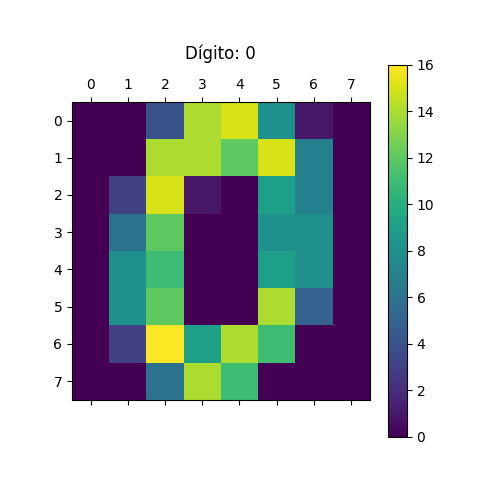
\includegraphics[width=57.5mm]{imgs/sample1.png}}
  \subfigure[Instancia correspondiente al 9]{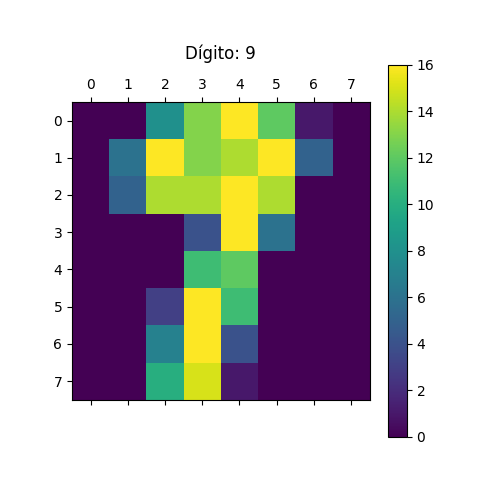
\includegraphics[width=57.5mm]{imgs/sample2.png}}
  \subfigure[Instancia correspondiente al 8]{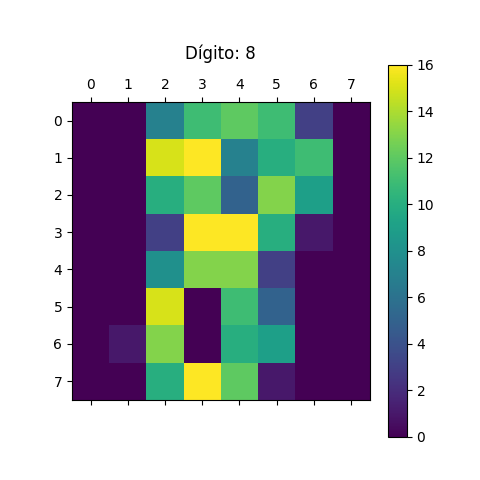
\includegraphics[width=57.5mm]{imgs/sample3.png}}
  \caption{Algunas instancias de los datos}
  \label{fig:samples}
\end{figure}

La población $X$ constituye el conjunto de vectores de 64 enteros
entre 0 y 16 que representan la cuadricula resultante de aplicar la
trasformación antes comentada; el conjunto de clases $Y$ constituye
los posibles dígitos: 0,1,2,3,4,5,6,7,8,9; y la función objetivo $f$
es la que asigna a cada vector de $X$ la clase del dígito que
representa.

Cabe preguntarnos si con los datos que tenemos podemos entrenar un
buen modelo, pues se ha perdido parte de la información al agrupar los
bits por cuadrículas. Para ello, podemos usar la función PCA
(Principal Component Analysis) para proyectar las dos características
que más me ayudan a distinguir los datos. Luego partimos de esa
proyección y aplicamos algoritmo TSNE (T-distributed Stochastic
Neighbor Embedding) para proyectar los datos en dos dimensiones de
forma que para cada dato sus vecinos más cercanos queden proyectados
cerca. Ambos algoritmos se encuentran progamados en \textit{sklearn}.

\begin{figure}[H]
  \centering
  \subfigure[Proyección 2D mediante PCA]{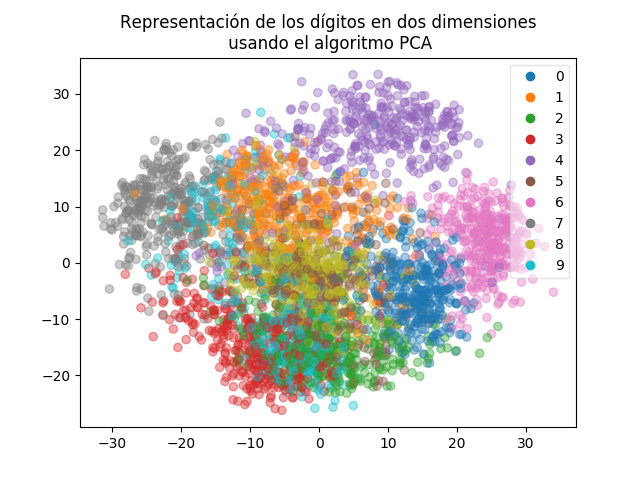
\includegraphics[width=87mm]{imgs/2dPCA.png}}
  \subfigure[Proyección 2D mediante T-SNE]{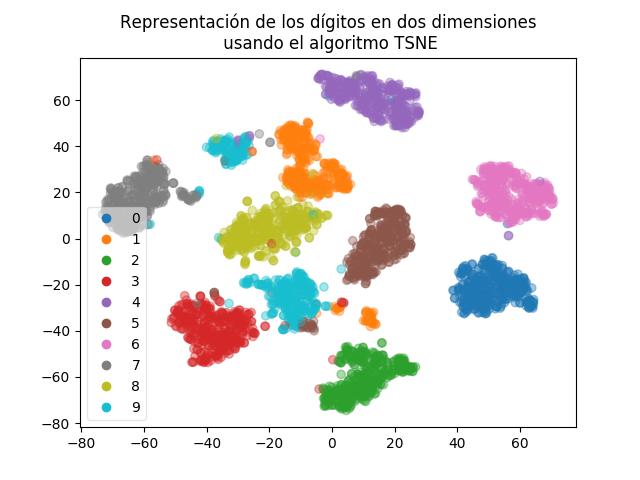
\includegraphics[width=87mm]{imgs/2dTSNE.png}}
  \caption{Visualización en 2D de los datos}
  \label{fig:2D-projection}
\end{figure}
\vspace{-4mm}

Sólo con las características principales ya podemos discernir
ligeramente entre los datos de diferentes clases. Y si tenemos en
cuenta todas ellas, los dígitos correspondientes a la misma clase se
encuentran bastante agrupados exceptuando algunas instancias sueltas.


\subsection{Conjuntos de training y test}

Los datos que nos proporcionan vienen ya separados en conjuntos de
training y test, y es importante que mantengamos esta división.

El motivo es que los datos de training corresponden a dígitos hechos a
mano por 30 personas diferentes y los datos de test a los de otras 13
personas.

Siempre es importante que en training y en test se utilicen conjuntos
disjuntos de datos para que $E_{test}$ sea un estimador de $E_{out}$
lo más representativo posible. Pero además en este problema es
importante que los dígitos usados en test estén hechos por personas
diferentes a las que generaron los dígitos de train, ya que es
presumible que el modelo reconozca mejor los dígitos trazados por las
mismas personas que trazaron los dígitos de entrenamiento.

Este hecho provoca que la estimación de $E_{out}$ realizada con
Cross-Validation sea demasiado optimista, por ser los datos de
validación correspondientes a las mismas personas que los de
entrenamiento. \label{cv-optimistic}

No separamos un conjunto de validación, ya que para decidir cuál es el
mejor modelo usaremos validación cruzada.

\subsection{Clases de funciones a usar y Preprocesamiento}

La clase de funciones que usaremos son los polinomios de grado 2, ya
que permiten obtener un modelo mucho más complejo y potente que
utilizar simplemente características lineales. Para añadir
características polinomiales usamos PolynomialFeatures.

El motivo por el que presento esta sección junto con procesamiento es
que la introducción de características polinomiales eleva el número de
variables al grado del polinomio, esto es computacionalmente costoso y
provoca que acabemos con demasiadas características. De hecho,
introducir características polinómicas de grado mayor que 2 es ya
demasiado costoso, por lo que no usamos grados más altos. Por este
motivo he decidido añadir la indroducción de características
polinomiales al preprocesamiento.

Para el preprocesamiento, creamos un Pipeline que primero elimina con
Variance Threshold las características con varianza menor que un
umbral, en este caso 0.005. Estas características apenas ayudan a
distinguir las instancias de la muestra. En segundo lugar añade
características de grado 2, ahora el número de características es
igual al cuadrado de las que quedaban tras la primera selección en
lugar de $64^2$. A continuación, realiza una estandarización con
StandardScaler y escala las variables para dejar todas con media 0 y
varianza 1. Por último utiliza otra vez PCA, pero esta vez en lugar de
proyectar un número fijo de variables, selecciona el menor número
posible que expliquen cierto porcentaje de la variabilidad de la
muestra, en este caso un 97.5\%.

Ajustamos el Pipeline con los datos de train y aplicamos las
transformaciones tanto a los de train como a los de test. Partíamos de
64 características y nos quedamos con 312. Teniendo en cuenta que
$64^2=4096$, sacrificando un pequeño porcentaje de la información
nos quedamos con un conjunto de variables bastante manejable.

Tanto el objeto Pipeline como los que realizan cada paso del
preprocesado se encuentran en \textit{sklearn}.

Para apreciar el resultado del preprocesado podemos visualizar la
matriz de coeficientes de correlación de Pearson, que indica la medida
en que unas características determinan otras. Si una característica
está determinada por el resto, se podría eliminar sin perder
información. Por tanto interesa que esta matriz sea diagonal, que cada
variable se determine únicamente a ella misma.

\vspace{-4mm}
\begin{figure}[H]
  \centering
  \subfigure[Antes del preprocesado]{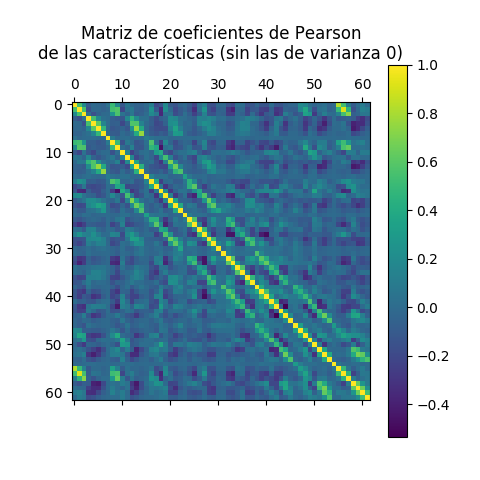
\includegraphics[width=87mm]{imgs/pearsonRaw.png}}
  \subfigure[Después del preprocesado]{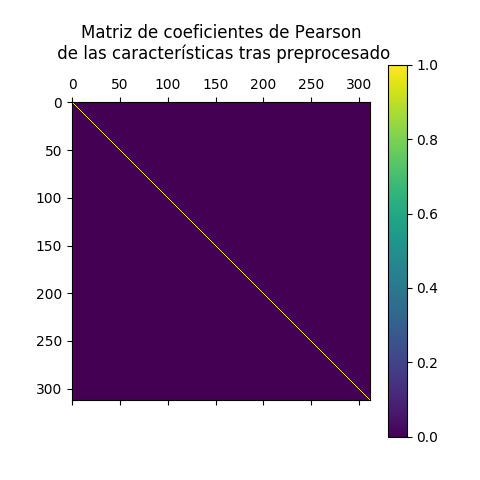
\includegraphics[width=87mm]{imgs/pearsonPre.png}}
  \caption{Matrices de coeficientes de correlación de Pearson}
  \label{fig:pearson}
\end{figure}
\vspace{-4mm}

Como podemos ver, fuera de la diagonal todos los coeficientes son
practicamente 0 como queríamos.

\subsection{Métricas}

Mirando el fichero \texttt{opdigits.names} percibimos que el número de
ejemplos de cada clase está balanceado tanto en training (entre 376 y
389) como en test (entre 174 y 183). En esta situación, la precisión
(accuacy, la proporción de elementos bien clasificados) es un métrica
adecuada de la bondad del modelo, además de fácil de interpretar.

Ésta será la métrica que estimaremos con validación cruzada y
compararemos con la que consiga en el conjunto de test.

También podemos visualizar la matriz de confusión (figuras
\ref{fig:conf-train} y \ref{fig:conf-test}). Es una matriz cuadrada de
orden el número de clases con números naturales como entradas, en la
que el valor de la posición $(i,j)$ representa el número de ejemplos
de la clase $i$-ésima que han sido clasificados por el modelo como
elementos de la clase $j$-ésima. Claramente interesa que la matriz de
confusión sea diagonal, ya que las entradas de la forma $(i,i)$
representan éxitos a la hora de clasificar y las entradas $(i,j)$ con
$j\neq i$ representan errores. De hecho, la accuracy se obtiene
dividiendo la traza de la matriz de confusión (el número de ejemplos
bien clasificados) entre el número total de ejemplos.

\subsection{Técnica de ajuste del modelo}

Aunque la métrica usada es la precisión, el modelo que usamos es el de
Regresión Logística Multietiqueta para estimar la probabilidad de
pertenencia a cada clase (la regla de clasificación será SoftMax),
minimizamos la Pérdida Logarítmica. \vspace{-2mm}
\[E(\textbf{w})=E(\textbf{w}_1,\ldots,\textbf{w}_K)=\frac{-1}{N}\sum_{n=1}^N\sum_{k=1}^{K}y_{nk}\ln\sigma(\textbf{w}_k^T \textbf{x}_n)\]
Donde cada $\textbf{w}_k$ es la fila $k$-ésima de una matriz de pesos
\textbf{w} de dimensión $K\times d$, con $K$ el número de clases (10)
y $d$ el número de características (312). Y las etiquetas $y_n$ están
codificadas como vectores one-hot ($y_{nk}=1$ si $y_n$ corresponde a
la clase $k$ y 0 en caso contrario).

Para minimizar esta función de pérdida utilizamos el algoritmo de
Gradiente Descendente Estocástico, en otras ocasiones ya hemos
comprobado su eficiacia a la hora de minimizar este tipo de funciones.
De hecho el motivo de que usemos esta función de pérdida y no la
proporción de fallos (1-accuracy) es la comodidad que tiene esta
función para minimizarla con esta técnica. Puedo calcular fácilmente
el gradiente respecto a cada una de las filas de la matriz \textbf{w}.\vspace{-2mm}
\[\nabla_{\textbf{w}_j}E(\textbf{w}_1,\ldots,\textbf{w}_K)=\frac{1}{N}\sum_{n=1}^N(\sigma(\textbf{w}_j^T \textbf{x}_n)-y_{nj})\textbf{x}_n\]\vspace{-4mm}

Necesito elegir un learning rate $\eta$ y un tamaño de minibatch
adecuados, estos son hiperparámetros del modelo que discutieremos más
adelante. El vector de pesos inicial es otro hiperparámetro que
fijaremos como el vector nulo por simplicidad.

\subsection{Regularización}

Las funciones cuadráticas que hemos introducido añaden un número
elevado de características y bastante complejidad al modelo, lo que lo
hace propenso al sobreajuste. Para evitar esto, debemos introducir
algún tipo de regularización.

En el preprocesado hemos eliminado bastantes atributos que no
aportaban apenas información sobre la variabilidad de la muestra,
luego cabe esperar que la mayoría de atributos que hemos seleccionado
sean relevantes. Es por ello que utilizaremos la Regularización Ridge,
reduciendo el cuadrado de la norma euclídea o norma de Frobenius de la
matriz de pesos \textbf{w}. La función de pérdida queda ahora
\vspace{-2mm}
\[E_{aug}(\textbf{w})=E(\textbf{w})+\lambda
  \|\textbf{w}\|_2^2\]\vspace{-2mm} donde
$\|\textbf{w}\|_2^2=\sum\limits_{k=1}^K\sum\limits_{j=1}^d
\textbf{w}_{kj}^2$ y $\lambda$ es un hiperparámetro del modelo sobre
el que hablaremos más adelante.

Esta fórmula es fácil de derivar, obteniendo \vspace{-2mm}
\[\nabla_{\textbf{w}_j}E_{aug}(\textbf{w})=\nabla_{\textbf{w}_j}E(\textbf{w})+\lambda 2\textbf{w}_j\]

\subsection{Modelos}

Como ya hemos comentado, usaremos un modelo de Regresión Logística
multiclase, ya que es el más adecuado de los modelos lineales que
conocemos para resolver un problema de clasificación no binario.

El modelo nos permite estimar para una instancia la probabilidad de
pertenencia a cada clase $j=1,\ldots,K$ mediante la fórmula:
\[P(y=j|\textbf{x})=\frac{e^{\textbf{w}_j \textbf{x}}}{\sum_{k=1}^K
    e^{\textbf{w}_k \textbf{x}}}\] A la hora de predecir utilizaremos
la regla SoftMax, que para una instancia \textbf{x} predice la
clase con mayor probabilidad.

Para aprovechar varias funcionalidades de \textit{sklearn},
implementamos nuestro propio objeto estimador (heredando de la clase
BaseEstimator) que depende de los hiperparámetros que hemos comentado
anteriormente. Debemos implementar como mínimo los métodos
\texttt{fit} y \texttt{predict}, \texttt{fit} recibe los datos de
entrenamiento y ajusta la matriz de pesos \textbf{w} minimizando la
Pérdida Logarítmica aumentada con SGD; \texttt{predict} recibe un
conjunto de ejemplos y aplica la regla SoftMax para determinar la
clase a la que pertenece cada uno.

Para evitar que el entrenamiento sea computacionalmente muy costoso,
he limitado el número de evaluaciones totales a 50000 para el SDG, a
la hora de aprender los datos se agrupan según el tamaño de
minibatch. Esto quiere decir que si el tamaño de minibatch es el
doble, se realizarán la mitad de iteraciones.

Esto no significa que no tengamos que discutir sobre el mejor modelo a
usar, ya que el modelo depende de varios hiperparámetros que
determinan su comportamiento y debemos estimar valores adecuados para
ellos.

\subsection{Estimación de hiperparámetros y selección del modelo}

Para decidir el mejor modelo debemos estimar los hiperparámetros, para
ello utilizamos GridSearchCV, que realiza una búsqueda exhaustiva en
rejilla probando todas las combinaciones de hiperparámetros en un
rango que determinamos. Para decidir qué combinación de parámetros es
mejor implementamos el método \texttt{score} en nuestro estimador, que
calcula el accuracy sobre un conjunto de datos. El algoritmo evalúa
cada combinación usando Cross Validation con 5 subdivisiones, esto es
tremendamente costoso (incluso paralelizando) por lo que lo omitimos
en la versión final del código (se controla con la variable booleana
PARAMSELECT).

Tras algunas horas de búsqueda, la combinación que mejor score ha
presentado entre las que he probado es $\lambda=0.007391304347826088$,
$\eta=0.001$, tamaño de minibathch = 1. Parece que lo más efectivo es
hacer un gran número de iteraciones con un sólo dato y una tasa de
aprendizaje baja. Con estos hiperparámetros, la precisión media de las
5 validaciones ha sido 0.9675642473394245, más que aceptable.

Por tanto, fijamos estos hiperparámetros y seleccionamos éste como el
mejor modelo. Primero medimos su efectividad sobre el conjunto de
training.

Pérdida logarítmica (aumentada) en la muestra: 0.04396861238743053 \\
Precisión sobre train: 0.9895370128171593

Matriz de confusión en la prueba sobre el conjunto de entrenamiento:
\vspace{-4mm}
\begin{figure}[H]
  \centering
  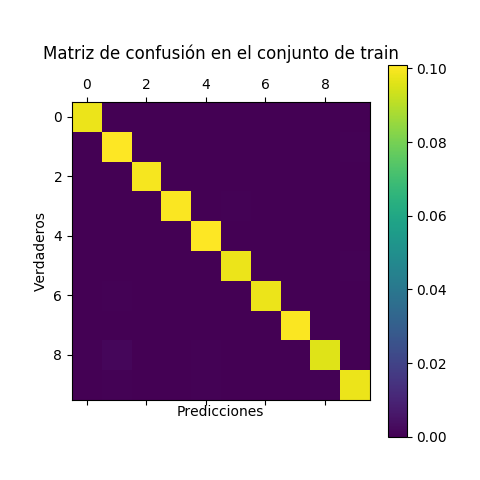
\includegraphics[width=100mm]{imgs/conf-train.png}
  \caption{Matriz de confusión en la prueba con los datos de
    entrenamiento}
  \label{fig:conf-train}
\end{figure}
\vspace{-4mm}

Tiene una precisión muy cercana a 1, más que su score en la selección
de modelos, ya que estos datos son los que he usado para entrenar el
modelo. La matriz de confusión es prácticamente diagonal, falla sobre
todo en algunas instancias de los dígitos 8 y 9 que ha clasificado
como unos.

\subsection{Estimación de $E_{out}$ por validación cruzada y
  comparación con $E_{test}$}

En lugar de error he considerado la precisión, que es una medida de
bondad. Usando la función \texttt{cross\_val\_score} de
\textit{sklearn} obtenemos una estimación por validación cruzada de la
precisión del modelo. Realiza 10 subdivisiones del conjunto de
entrenamiento, por lo que necesita entrenar y validar 10 veces. Este
proceso es algo lento, pero la función permite paralelizarlo. La
precisión media que he obtenido en las 10 validaciones es
$E_{cv} = 0.9764602955449538$ (este valor varía entre ejecuciones).

Primero sacamos tres muestras aleatorias del conjunto de test, en
las tres el modelo ha dado con la clase correcta.

\vspace{-5mm}
\begin{figure}[H]
  \centering
  \subfigure[Instancia correspondiente al 3]{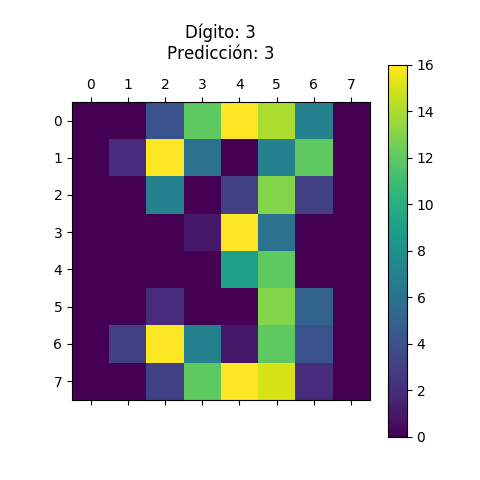
\includegraphics[width=57.5mm]{imgs/test1.png}}
  \subfigure[Instancia correspondiente al 5]{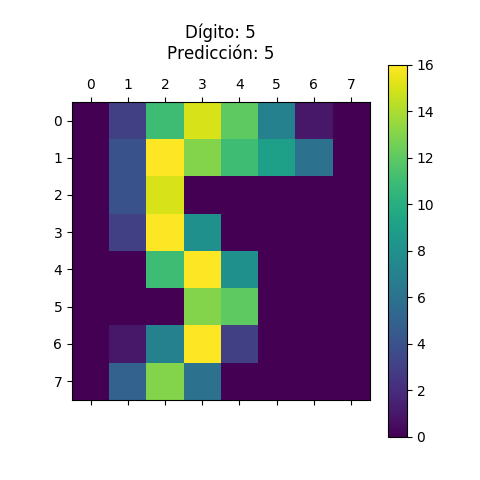
\includegraphics[width=57.5mm]{imgs/test2.png}}
  \subfigure[Instancia correspondiente al 0]{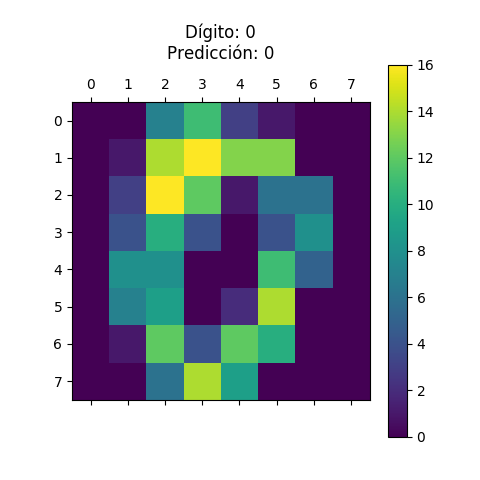
\includegraphics[width=57.5mm]{imgs/test3.png}}
  \caption{Algunas instancias de los datos}
  \label{fig:tests-samples}
\end{figure}
\vspace{-5mm}

Evaluamos ya el modelo sobre el conjunto de test.

Pérdida logarítmica (aumentada) en test: 0.08595584205059877 \\
Precisión sobre test: 0.9671675013912076

Matriz de confusión en la prueba sobre el conjunto de test:
\vspace{-4mm}
\begin{figure}[H]
  \centering
  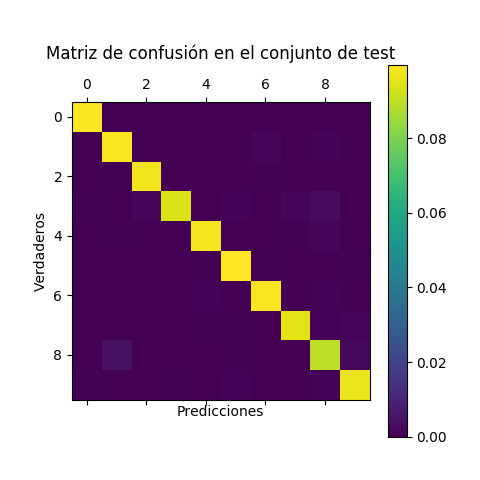
\includegraphics[width=100mm]{imgs/conf-test.png}
  \caption{Matriz de confusión en la prueba con los datos de test}
  \label{fig:conf-test}
\end{figure}
\vspace{-4mm}

La precisión obtenida sobre el conjunto de test es ligeramente menor
que la estimación realizada por validación cruzada. Esto se debe a la
razón que comenté en la sección \ref{cv-optimistic} de que la
validación y el entrenamiento se realizan sobre datos correspondientes
a dígitos trazados por las mismas 30 personas y los dígitos tienden a
ser más parecidos entre ellos que los de test, que están trazados por
otras 13 personas diferentes.

No obstante, la precisión obtenida es aceptable. Tampoco podemos
optar a mucha más precisión puesto que hemos renunciado a algo más del
2.5\% de información sobre la variabilidad de la muestra para
simplificar los datos durante el preprocesamiento.

El modelo falla sobre todo al clasificar algunos ochos como unos, lo
que también ocurría en la prueba con los datos de entrenamiento.

\subsection{Conclusiones}

Para comparar utilizamos el clasificador por KNN de
\textit{sklearn}, que predice la clase de un elemento según la clase
que más abunde entre sus 5 vecinos más cercanos del conjunto de
entrenamiento.

En el fichero \texttt{opdigits.names} asegura que este algoritmo
consigue una precisión mayor que la de nuestro modelo, lo
comprobaremos.

Sobre los datos procesados de test el algoritmo ha obtenido una
precisión de 0.9577072899276572, algo más baja que la de mi modelo.
Esto nos indica que sobre los datos procesados nuestro modelo es más
que decente.

Sin embargo, sobre los datos de test sin procesar el algoritmo KNN ha
obtendio una precisión de 0.9788536449638287 (corresponde a lo
indicado en \texttt{opdigits.names}), más alta que nuestro
clasificador por regresión logística. Esto podría significar que hemos
cometido un error al preprocesar los datos, pero tras probar nuestro
modelo de regresión logística con los datos sin preprocesar concluimos
que el preprocesado supone una importante mejora (accuracy Cross
Validation: 0.9495174497286509, accuracy test: 0.9454646633277685),
luego el preprocesar los datos ha sido una decisión acertada de cara a
la eficacia del modelo lineal usado.

Concluimos que el modelo elegido no es el mejor, pero tiene buena
calidad. Sí que ha proporcionado la mejor precisión entre las
distintas posibilidades exploradas (variando los hiperparámetros).

En un caso real de que nos hubiesen encargado un modelo que resolviese
este problema hubiesemos proporcionado este modelo con la precisión
obtenida por validación cruzada. Tendríamos que advertir de que esa
precisión se ha estimado usando un conjunto de validación disjunto del
de entrenamiento, pero con datos correspondientes a números trazados
con las mismas personas, y que esto podría provocar que la precisión
del modelo sea menor en datos correspondiéntes a dígitos trazados por
personas distintas. De no haber hecho esta advertencia y limitarnos a
devolver el modelo y la estimación de la precisión por validación
cruzada, habríamos cometido el error de ofrecer una estimación de la
bondad del modelo demasiado optimista.

Para poder probar la bondad real del modelo hemos necesitado el
conjunto de test, que es probable que en un problema real no
tuviésemos. Se podría paliar este problema si en los datos
proporcionados nos proporcionasen los datos separados por la
persona que trazó el dígito, pero no era el sido el caso.

\section{Predicción de crímenes violentos per cápita}

\subsection{Problema}

Queremos predecir el número de crímenes violentos por cada 100.000
habitantes en distantas comunidades. Disponemos de un conjunto de
datos que incluye variables como porcentajes de población en un rango
de edad, con un determinado nivel de estudios, perteneciente a cierta
raza, que ha emigrdo\ldots También sobre las rentas, el desempleo, el
número de policías por cada $x$ habitantes\ldots

Claramente podemos plantear este problema como un problema de
Regresión Lineal y entrenar un modelo para predecir la variable
objetivo con datos de los que disponemos.

Todas las variables (numéricas) han sido normalizadas entre 0 y 1,
manteniendo su distribución y simetría/asimetría. La normalización
colapsa los outliers a 0 o 1 (según si estan muy por debajo o por
encima del resto), por lo que no tenemos que preocuparnos por la
existencia de outliers. Sí debemos tener en cuenta que esta
normalización preserva los ratios entre valores del mismo atributo,
pero no entre atributos, no tiene sentido comparar dos atributos
diferentes.

Podemos encontrar toda la información sobre los datos en el fichero
\texttt{communities.names}, esto lo tendremos en cuenta para gestionar
el problema de la existencia de valores perdidos. En total hay 127
variables + la variable objetivo, de estas 127 sólo hay 122
predictivas, así que desechamos el resto.

Entre las variables restantes, 22 de ellas presentan un gran
porcentaje (84\%) de valores perdidos, tendremos que decidir qué
hacemos con ellas.

La población $X$ constituye el conjunto de valores normalizados entre
0 y 1 de las variables correspondientes a una comunidad; $Y$ es el
conjunto de posibles números de crímenes violentos normalizados (esto
no quiere decir que estén entre 0 y 1, como explicamos en el siguiente
párrafo); y la función objetivo $f$ es la que asigna a cada vector de
$X$ el número de crímenes violentos en la comunidad que representa
normalizado entre 0 y 1.

Con esta normalización sobre la variable objetivo debemos tener
cuidado, ya que ante la aparición de un nuevo dato para el cual el
modelo predice un índice de criminalidad superior al mayor de entre
las comunidades de los datos que tenemos (predeciría $y>1$) puede no
ser adecuado interpretar el valor como 1. Ya que esto desecha
información sobre comunidades con mayor tasa de crímenes violentos que
las de los datos. Es por ello que permitiremos que nuestro modelo
prediga valores de $y$ superiores a 1.

Tras gestionar los valores perdidos en el preprocesamiento, podemos
visualizar los datos. He usado la misma técnica que antes: PCA + TSNE

\vspace{-4mm}
\begin{figure}[H]
  \centering
  \subfigure[Proyección 2D mediante PCA]{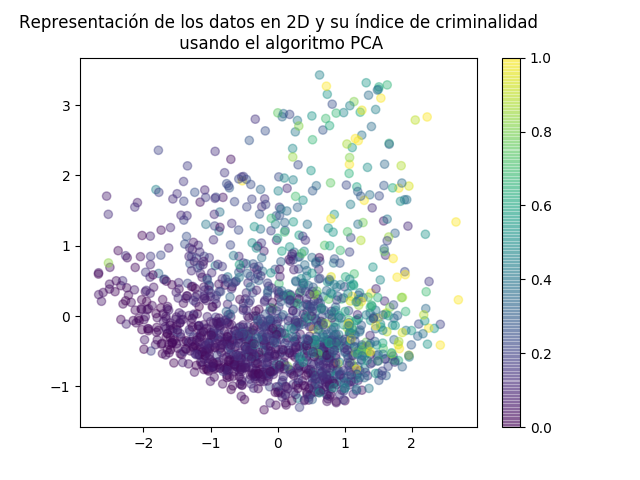
\includegraphics[width=87mm]{imgs/com_2dPCA.png}}
  \subfigure[Proyección 2D mediante T-SNE]{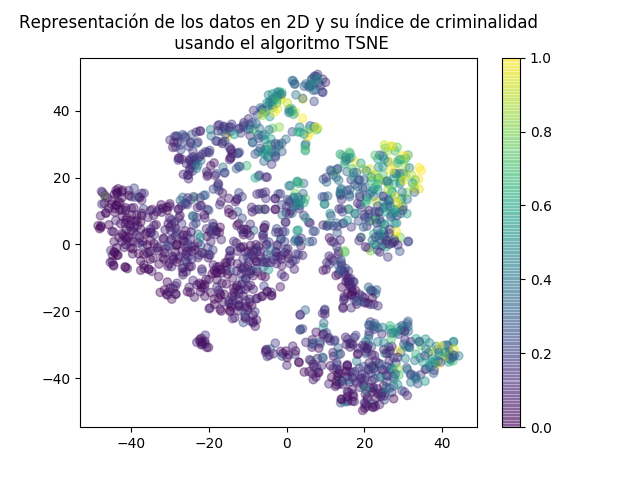
\includegraphics[width=87mm]{imgs/com_2dTSNE.png}}
  \caption{Visualización en 2D de los datos}
  \label{fig:com_2D-projection}
\end{figure}
\vspace{-4mm}

Se aprecia que los datos correspondientes a comunidades con diferente
índice de criminalidad no están demasiado entremezclados. Al ser la
variable a predecir de carácter continuo, no podíamos esperar que los
datos estuviesen tan separados como en el problema anterior. Pero
tenemos una transición gradual entre los datos correspondientes a
instancias con distinto índice de criminalidad (variable objetivo).

\subsection{Conjuntos de training y test}

A diferencia del otro problema, en este caso no se nos proporciona un
conjunto de test separado, por lo que debemos extraerlo del conjunto
de train. Lo hacemos con la función \texttt{train\_test\_split} de
\textit{sklearn}, y elegimos 75\% de datos para train y 25\% para test
de forma aleatoria.

\subsection{Clases de funciones a usar y Preprocesamiento}

Por la misma razón que antes usamos polinomios de grado 2 y los
introducimos en medio del preprocesamiento.

Además de eliminar las variables no predictivas, realizamos las
siguientes tareas:

Primero debemos decidir qué hacer con los valores perdidos, puesto que
no son demasiadas variables las que presentan valores perdidos y en
ellas la proporción de valores perdidos es relativamente alta (84\%),
mi primera decisión fue eliminar dichas variables, quedandome con 100.
Para ello he usado la función \texttt{dropna} de \texttt{pandas}, para
desechar los atributos con más del 50\% de valores perdidos. El Error
Cuatrático Medio obtenido con validación cruzada bajo esta decisión ha
sido $E_{cv} = 0.02356922860102622$.

En el caso de no eliminarlas (o por si queda alguna con el 50\% o
menos de valores perdidos), tenemos que estimarlas de alguna
forma. Para ello usaremos KNNImputer de \texttt{sklearn}, que estima
cada valor perdido promediando los de los 5 vecinos (que tienen el
valor) más cercanos en la distancia euclídea (atendiendo a la
características sin valores perdidos), da más peso a los vecinos más
cercanos. Aplicamos esto tanto en train (fit y transform) como en test
(sólo transform).

Si en lugar de eliminar las características con demasiados (>50\%)
datos perdidos, las interpolamos con KNNImputer, el ECM que obtenemos
en validación es $E_{cv} = 0.027620319480671656$, por lo que
mantenemos la decisión de eliminarlas.

A continuación aplicamos (también en un Pipeline) las mismas
transformaciones que el problema anterior: eliminamos variables con
baja varianza (<0.005), añadimos características polinomiales de grado
2, escalamos a media 0 y varianza 1 y elegimos el menor número de
variables que expliquen el 99\% de la variabilidad de la distribución.
Nos quedamos con 260 atributos, perfectamente manejable.

Al igual que antes, visualizamos la matriz de coeficientes de
correlación de Pearson antes (pero ya sin valores perdidos) y después
del preprocesamiento. Comprobamos que queda diagonal.

\vspace{-4mm}
\begin{figure}[H]
  \centering
  \subfigure[Antes del preprocesado]{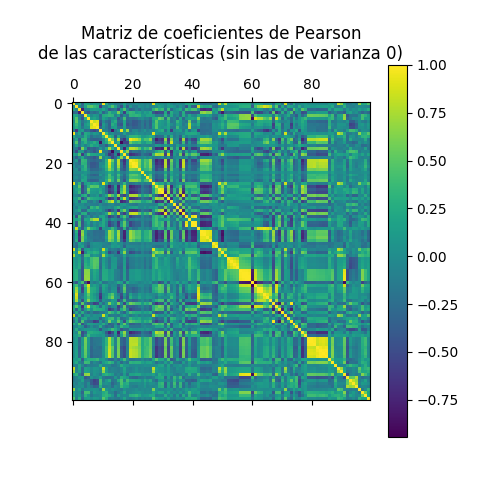
\includegraphics[width=87mm]{imgs/com_pearsonRaw.png}}
  \subfigure[Después del preprocesado]{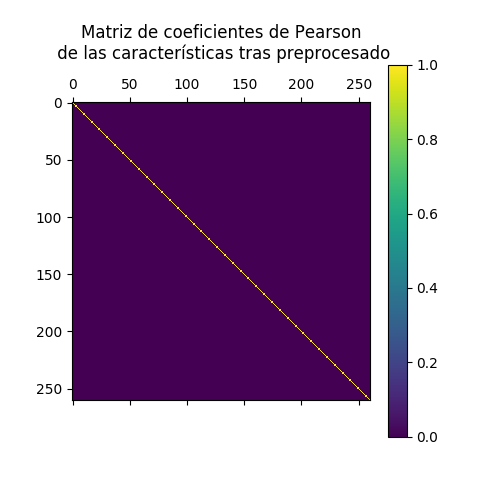
\includegraphics[width=87mm]{imgs/com_pearsonPre.png}}
  \caption{Matrices de coeficientes de correlación de Pearson}
  \label{fig:com_pearson}
\end{figure}
\vspace{-4mm}

\subsection{Métrica}

La función que minimizaremos es el error cuadrático medio (MSE, mean
squared error), también será la función en la que basaremos nuestra
elección de cuál es el mejor modelo en la fase de validación.

Preferimos esta función al error absoluto medio (MAE, mean absolute
error) porque, aunque es cierto que el MAE es más robusto ante los
outliers, en este caso disminuye su influencia al haber sido
normalizados. El MSE es más adecuado cuando queremos tener en cuenta
cada uno de los datos de los que disponemos, no permite que algún dato
tenga error demasiado alto a cambio de predecir otro con más exactitud.

No obstante, aunque basemos en el MSE la elección del modelo,
estudiamos también el coeficiente de determinación $R^2$ y lo
comparamos con el de otros modelos a la hora de sacar conclusiones
respecto a la calidad del modelo elegido. Debido a su fácil
interpretación: la proporción de la variabilidad de la distribución
que puede explicarse por el modelo.

\subsection{Técnica de ajuste del modelo}

Para minimizar el MSE, podemos usar el SGD o la pseudoinversa. Nos
decantamos por esta última debido a que la matriz a invertir no tiene
un orden excesivamente alto (tenemos 260 características + la columna
de unos) y las operaciones matriciales en \textit{numpy} están muy
optimizadas. Además, este algoritmo permite calcular el vector de
pesos \textbf{w} que anula el gradiente de la función de error de
forma casi exacta y no precisamos estimar hiperparámetros como son el
learning rate, el tamaño de minibatch y los pesos
iniciales. Obtenemos:
$\textbf{w}=\textbf{X}^+ \textbf{y}=(\textbf{X}^T
\textbf{X})^{-1}\textbf{X}^T \textbf{y}$

\subsection{Regularización}

Al igual que en el problema anterior, gracias al preprocesamiento
podemos esperar que la mayoría de atributos sean relevantes, por lo
que utilizaremos Regularización Ridge. Esto modifica la fórmula de la
pseudoinversa anterior, para tener en cuenta la penalización por
regularización. Obteniendo
$\textbf{w}_{reg}=(\textbf{X}^T \textbf{X}+\lambda I)^{-1}\textbf{X}^T
\textbf{y}$ donde $I$ es la matriz identidad de orden $d+1$ ($d$ es el
número de características) y $\lambda$ un hiperparámetro del modelo
que debemos discutir más adelante.

\subsection{Modelos}

El modelo que usaremos será el de Regresión Lineal para minimizar el
Error Cuadrático Medio, el más adecuado entre los modelos lineales que
conocemos para este problema (predecir una variable continua a partir
de otro conjunto de variables). Como ya hemos comentado, lo
ajustaremos con el algoritmo de la pseudoinversa añadiendo
regularización.

Para este problema también he creado un objeto estimador de
\textit{sklearn} que ajusta el vector de pesos \textbf{w} mediante
pseudoinversa (con regularización) para el método \texttt{fit} y
realiza el producto escalar de un vector de atributos de entrada
\textbf{x} por \textbf{w} para predecir la variable objetivo en el
método \texttt{predict}.

En este caso sólo tenemos un hiperparámetro
($\lambda$, la penalización de la regularización) que estimaremos de
la misma forma que en el problema anterior.

\subsection{Estimación de hiperparámetros y selección del modelo}

Ajustando modelo mediante pseudoinversa ...
ECM aumentado sobre la muestra: 4.323467888321191
ECM sobre la muestra: 0.013243601309686465
$R^2$= 0.7517257860345214


\end{document}

\subsection{Estimación de $E_{out}$ por validación cruzada y
  comparación con $E_{test}$}

Ecv = 0.02356922860102622


Selecciono un elemento aleatorio de test
Objetivo: 0.32
Predicción: 0.2428077121087347
Diferencia: -0.07719228789126531

--- Pulsar tecla para continuar ---

Selecciono un elemento aleatorio de test
Objetivo: 0.29
Predicción: 0.37131158436817296
Diferencia: 0.08131158436817298

--- Pulsar tecla para continuar ---

Selecciono un elemento aleatorio de test
Objetivo: 0.09
Predicción: 0.13948687744365962
Diferencia: 0.04948687744365962

--- Pulsar tecla para continuar ---

Selecciono un elemento aleatorio de test
Objetivo: 0.2
Predicción: 0.3688994745851004
Diferencia: 0.1688994745851004


ECM aumentado sobre el test: 4.329183968372332
ECM sobre el test: 0.018959681360827634
R²= 0.6671865221163271

\subsection{Conclusiones}


Comparación con KNN
ECM sobre test: 0.02153277755511022
KNN R²= 0.622019038705042


Comparación con Random Forest
ECM sobre test: 0.023047872064128255
KNN R²= 0.595423450769131

\end{document}
